\documentclass[12pt,twocolumn]{article}
\usepackage{amsmath}
\usepackage{amssymb}
\usepackage{graphicx}
\usepackage{fancyhdr}
\usepackage{enumerate}
\usepackage{titlesec}
\usepackage[colorlinks=true,urlcolor=blue]{hyperref}
\usepackage[top=1in, bottom=1in, left=0.8in, right=0.8in]{geometry}

% correct bad hyphenation here
\hyphenation{op-tical net-works semi-conduc-tor}


\begin{document}
%
% paper title
% Titles are generally capitalized except for words such as a, an, and, as,
% at, but, by, for, in, nor, of, on, or, the, to and up, which are usually
% not capitalized unless they are the first or last word of the title.
% Linebreaks \\ can be used within to get better formatting as desired.
% Do not put math or special symbols in the title.
\title{Money Moves the Pen: \\ Link Prediction in Congress Bill Co-Sponsorship Networks Using Political Donor Network Information}


% author names and affiliations
% use a multiple column layout for up to three different
% affiliations
\author{\textbf{Yi Zhong}, yizhon@stanford.edu \\\textbf{Eddie Chen}, yc4@stanford.edu}

% make the title area
\maketitle

% As a general rule, do not put math, special symbols or citations
% in the abstract
\begin{abstract}
We combined the campaign contribution records and congressional bill co-sponsorship data to construct a tri-partite graph, in order to model the money politics in the US Congress. We found that the US Congressional Politics is indeed a small world with collaboration resembling academic collaborations. More importantly, we modeled the bill co-sponsorship prediction as a link prediction problem, using attributes learned from campaign contribution networks. Result shows that using campaign networks is a good way to predict future in-office collaboration between legislators, especially with a supervised, decision-tree model. 
\end{abstract}
\section{Introduction}
Political collaboration is an important part of legislative life, and congress bill cosponsorships provide a rich source of information about the social network between legislators \cite{fowler2006connecting}, and serving as a proxy to understand legislators' "connectedness" and collaboration graph. Moreover, according to Mark Twain, "we have the best government that money can buy" - money and politics have already been intertwined. In this project, we applied social network analysis tools on political donation networks and congress bill cosponsorship networks, and framed our research problem as a link prediction task on congress bill cosponsorship networks using political campaign donation records for the US (Congress and Presidential Campaigns) with its network characteristics. We modeled and presented graph characteristics of the two political networks, and showed investigation results of link prediction using various supervised learning techniques for this project. We then compared models' performance to a naive baseline to come up with evaluations. 
\section{Related Work}
While there is a substantial amount of literature in studying the congress networks and the link prediction problem, no prior work exists on combining congress bill sponsorship network with campaign money networks and apply link prediction algorithms to the combined graph. Below, we review some of the state-of-the-art papers on this topic. 

\textbf{Fowler} in his \textit{Connecting the Congress: A Study of Cosponsorship Networks} \cite{fowler2006connecting} mapped the cosponsorship networks of all 280,000 pieces of legislation proposed in the U.S. House and Senate from 1973 to 2004, and reported out several interesting statistics about the resulting networks. He further proposed a measure of "connectedness" by looking at the frequency of cosponsorship and the number of cosponsors on each bill to estimate the social "distance" between legislators, and used "connectedness" as a proxy for legislative influence. While the paper has done an excellent exploration around America's political networks from an unique angle, it leaves more to be desired. He treated all the links as unweighted in the paper; but as he himself pointed out, some cosponsors are probably more important than others. Another downside of this paper is that it ignores the temporal aspects of the co-sponsorship network. It only looks at each Congress in this isolation without change over time. Yet, given the dynamic nature of bill writing and co-sponsoring, a study of how co-sponsorship network forms and evolves (link prediction) can reveal insight on how one can work on being more connected and more influential in legislative outcomes. 

\textbf{Dominguez} \cite{dominguez2005groups} examined the makeup of the Democratic and Republican party coalitions by analyzing the contribution patterns of elite donors (defined as  all individual donors who gave over \$200 to one of the two major political party committees in the 2003-2004 election cycle) and their network patterns. He showed that both parties are similar in their degree of centralization, with the party committees being the most central actors in the network. 

Both political donor networks (in the form of Super PACs) and Congress bill cosponsorships have been studied by students in CS224W before. In \textit{\textbf{Co-Authorship Networks in Congress}} \cite{perozo_garcia_banerjee_2016}, the authors looked at the impact of co-sponsorship on legislation success.  They used the network characteristics to predict future co-sponsorship, via \textbf{Supervised Random Walks and Triads}. While this past project provided a lot good ideas, it lacked a discussion on using other machine learning models, which can potentially yield good results, especially when the network is dense and Supervised Random Walks are known to perform well on sparse graphs.

In \textbf{\textit{Super-PAC Donor Networks}} \cite{moody_2015}, the author studied individual donors and their contributions to specifically Super PACs, a new form of political action committees that can raise unlimited sum of money for campaigns. The authored looked at community structures and other network characteristics for insights on partisan polarization. The author did not show how networks evolve over time, as donations might swing back and forth depending on which party is in power, and the change in donor demographics. 

For Link Prediction, \textbf{Liben-Nowell et al.} \cite{liben2007link} discusses similarity based methods for link prediction, and focuses on using network intrinsic traits to predict its future edge evolution. It explores a wide array of similarity measures (such as Common Neighbors, Jaccard's Index, Adamic/Adar, and Katz clustering, etc.) and compares their prediction accuracy among themselves and against a random predictor as baseline. However, the definition of node similarity is a nontrivial challenge, and it's likely that different networks would require different definition of node "proximity". Moreover, a lot of the similarity measures assume that the link itself indicated similarity between two nodes, which may or may not be true. 

\textbf{Al Hasan et al.} \cite{al2006link} models the link prediction problem as a supervised learning task, identifies a set of proximity, aggregated, and topological feartures, and applies common supervised algorithms like decision tree, SVM, $k$-NN, etc. It evaluates these different models using metrics such as accuracy, recall, F-values,etc. However, the paper skips entirely on hyper-parameter fine-tuning for the model of choice (SVM), likely because of the high accuracy it was able to achieve with its well selected features. Moreover, the paper landed luckily on a balanced data set with roughly equal numbers of positive and negative labels; yet for most tight-knit communities that resemble a "small world", labels are likely skewed, and we need to pay close attention to data selection for training, and probably considering techniques like down-sampling. 

\textbf{Backstrom et al} \cite{backstrom2011supervised} proposed a new hybrid solution in tackling link prediction problem. It uses Random Walks with Restarts (basically Personalized PageRank with one node) as a way to explore the network structure. It then looks at the node and edge attribute data to bias the random walk so that it will more often visit nodes to which creates edges in the future, in a direct and principled way and not to overfit. Yet, the paper only considers node and edge attribute data, and posits that such intrinsic structure likely reflects exogenous characteristics as well (in the Facebook friending example, one’s location/closeness in network to other people reflects the likelihood of people partying together and therefore adding on Facebook together). It’s unclear to me if this holds true in political networks, especially in the Congress, when politicians come from vastly different places all over the country and from different ideological allegiances as well.

The related work reviewed above provided a lot great ideas, and the most obvious one is perhaps to marry political donor network, congress bill co-sponsorship network, and link prediction together. Below, we present 3 creative contributions our project explored. 
\begin{enumerate}
\item \textbf{Model networks}: Both sections above deal with bipartite graphs, and our subject of study is a tripartitite graph consisting of donors, politicians and bills. Unlike Fowler \cite{fowler2006connecting}, we modeled networks as \textbf{undirected}, which is more compatible with existing link prediction literature. 
\item \textbf{Incorporate edge weights in supervised learning models}: Because our network of interest here carries a lot important information such as \textbf{donation amount}, We extended the abovementioned work by incorporating edge weights.  
\item \textbf{Compare features learned from graph to candidate information}: We ran models based on features learned from candidates' campaign donation networks versus models based on candidates' party and home state information, to understand what information is more predictive.
\end{enumerate}

\section{Method}
\subsection{Problem Statement}
Our project is made up of two parts: graph modeling, and link prediction. For graph modeling, we aim to construct a tripartite graph of political committees, legislators (we will ignore those failed to get elected to office), and the bills those legislators worked together on. A sample graph can be found in Figure \ref{fig_sim}. With the graph constructed, we provide a set of statistics and descriptions of the graph structure (including their one-mode projections, for both bills-legislators and committees-legislators subgraphs). After that, we construct a link prediction problem by dividing graph into different years of congress, and select the suitable years for model training and evaluation. Lastly, we report our learnings from the entire exercise. 

\begin{figure}
\centering
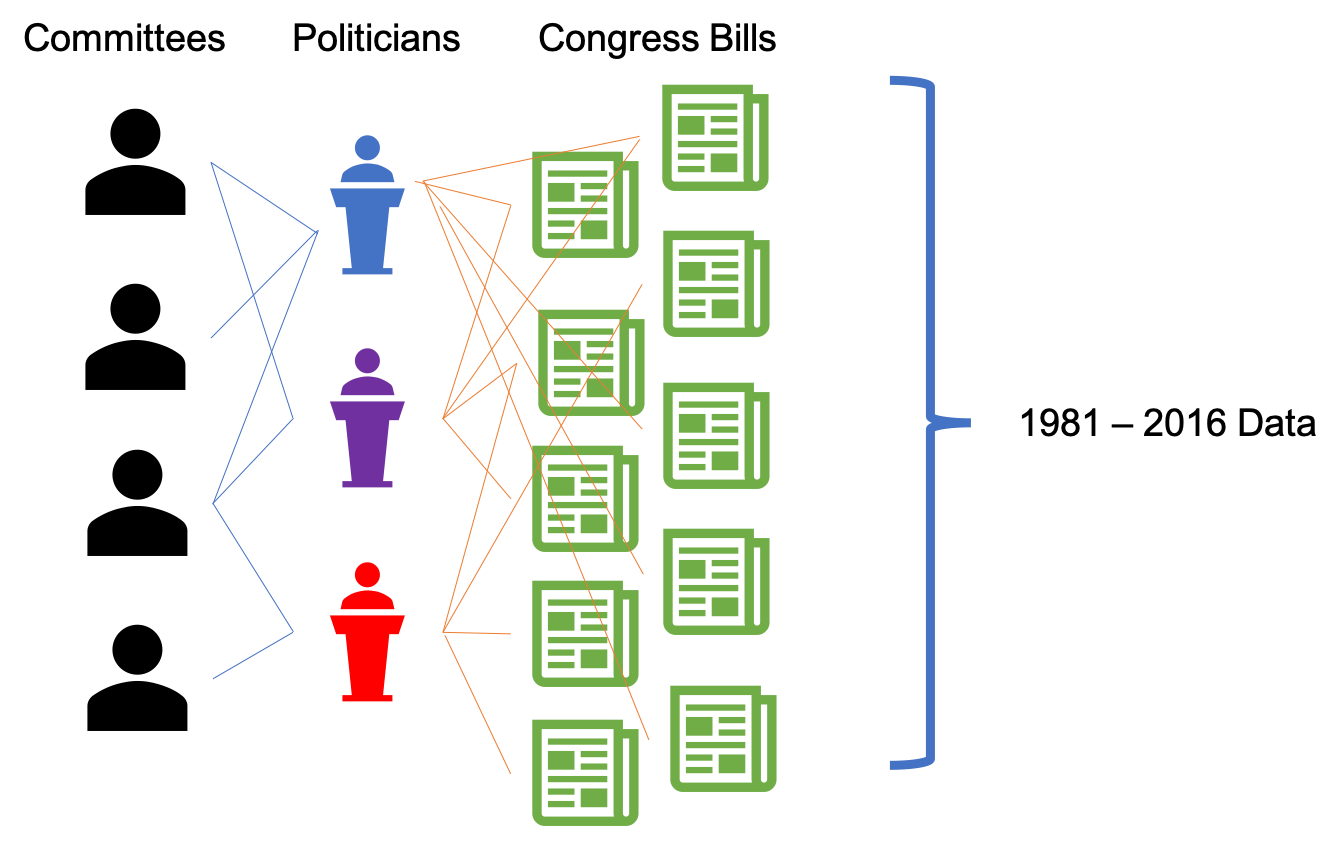
\includegraphics[width=\linewidth]{network_illustration2}
\caption{Illustration of the Congress Political Network}
\label{fig_sim}
\end{figure}

Practically, we hope our research can quantitatively answer the question: \textbf{Does donation in election affect collaboration in office?} Given a graph of congressional politicians and their campaign donations, we want to predict who will co-sponsor bills together as a form of political collaboration. Here we focus on congressional bill (including all resolutions, bills, and amendments) co-sponsorship because co-sponsorship is an observable signal, and tells us intuitively how much support one bill has and therefore how much clout the politician behind the bill has. 

This problem has obvious utility: it would be useful to keep the electorate informed of their elected representatives' political collaborations and alliances in the Congress, as well as indicate any changes or tendencies in politicians' stances on various issues. Moreover, for politicians, this information can be used as a guidance to seek more targeted co-sponsors, sparing them from wasting precious political capital and writing countless (and potentially spammy and ineffective) "Dear Colleagues" letters. 

\subsection{Data Preparation}
In this project, we used the campaign financial data provided by the Federal Election Committee\footnote{FEC Website data: \url{https://www.fec.gov/data/advanced/?tab=bulk-data} } from 1981 to 2016 (the 97th to the 114th Congress, including House, Senate and Presidential races). The bill co-authorship data is obtained from the Government Publishing Office's website for the same period. \footnote{\url{https://www.govinfo.gov/bulkdata/BILLS/115}}.  We have hosted our code repository at \url{https://github.com/yzhong94/cs224w-project/}. 

A large part of effort to date has been devoted to data cleaning. In particular, we have to join the campaign financial data, which uses FEC's Candidaite IDs, with the Congress bill data, which uses its own ID system, on legislators. Our approach is to first join by legislator's capitalized full first name + last name + state (abbreviation), which leaves out more than 100 legislators not being matched between the two datasets. A close examination reveals that some legislators go by nicknames in signing bills but have full legal names on the campaign financial records - for instance, Tom Lewis is actually Thomas Lewis, and James Cooper going by Jim; this is made worse by irregular nicknames too, such as Richard "Doc" Hastings. Some legislators go by their middle names, such as Raymond Eugene Green going by Gene Green, David Adam Smith by Adam Smith. To combat this, we first filtered out all the candidates not matched by the method above (capitalized full first name + last name + state abbreviation), and joined them together by capitalized full last name + state abbreviation, because people are very unlikely to have nicknames for their last names. After that, we created an Excel check function to alert us if we have one NodeID (from the bill data) maps to multiple different Candidate IDs (note: it's possible for a person to have two different Candidate IDs, which happens when this person ran for House first, then Senate later). We then manually inspected the flagged rows and kicked out false positives. In the end, we were able to find 1813 legislators/candidates from both the campaign financial record and the bill co-sponsorship data from 1981 to 2016. 

\subsection{Network Construction}
We constructed a tripartite network: committees, legislators, bills.  A committee can be a PAC, SuperPAC or party committee.  A legislator is an elected official in the Congress, which can be a senator or a representative. A bill is a draft of legislation that has been sponsored by a legislator and co-sponsored by others. To describe the whole graph, we include all years of data first (from 1981 to 2016), and then look at one term's data for an individual graph. 

Between committees and legislators, an undirected link is added if a committee donates to a legislator (we do not allow for multiple edges between two nodes). This way, we ended up having 1813 candidates with donations across the years. We aggregated the donation amounts between candidates and committees by year and preserved the sum as edge weights, to simplify multi-edges.  Between legislators and bills, an undirected link is added first if candidates appear on the bill as either an author or a co-sponsor. 

\subsection{Link Prediction}
After constructing the graph, we applied \textbf{supervised learning link prediction} on the bill co-sponsorship part of the tripartitite graph, \textbf{between politicians and bills}.

Formally, let $G(V,E)$ be our entire tripartitite graph with node set $V$ and edge set $E$, covering periods from $t_{start}$ to $t_{end}$. Let $t_0$ be an arbitrary time period between  $t_{start}$ to $t_{end}$. Our training and test graph pair will be $\{G_{t_{0}}, G_{t_{1}}\}$: we will train based on network characteristics found in the subgraph $G^{campaign}_{t_{0}}(V_{legislators}, V_{committees})$, and use that to predict edge formations among \textbf{the candidate nodes} in $G^{co-sponsor}_{t_{1}}(V_{legislators},V_{bills})$ where $V \in \{G_{t_{0}}, V_{legislators}\}$ (which is $V_{legislators, t_1}$). We can then repeat the process, run the best model on a new pair of graphs (for different years) as validation, and report the metrics for final evaluation. 

We frame our link prediction problem as follows: predict the link between legislators, where a link exists if two legislators cosponored a bill together, for a specific Congress term.  

We have constructed three link prediction models:
\begin{itemize}
    \item Naive baseline predictor: a baseline model based on graph density
    \item Legislator only predictor: a baseline model based on candidate attributes (party, state)
    \item Campaign only predictor: prediction model using features generated from campaign graph network attributes
\end{itemize}

\subsubsection{Naive baseline predictor}
We define our \textbf{naive baseline predictor} as follows: given a pair of nodes$v_1, v_2$, we will always predict there will be an edge between these two pairs, i.e. as a complete graph. This is computed for $G_{co-sponsor}$.  That is, $$Accuracy_{Naive Baseline} = \frac{2||E||}{||V|| \dot (||V|| - 1)} $$

Using the 100th Congress (1987 - 1988) as the training set and the 101th Congress (1989-1990) as the test set.  The baseline accuracy is calculated as $96,052/138,075= 0.695$ per above. 

\subsubsection{Legislator only predictor}
We define a second baseline using \textbf{legislator attributes only}.  \textbf{Features for link prediction all come from information about the legislators}.  There are two features: IsFromSameState, IsFromSameParty.

Formally, for every $E(V_{legislator,i},V_{legislator,j}$ in $G_{co-sponsor}$, IsFromSameState is 1 if $V_{legislator,i}$ and $V_{legislator,j}$ are from the same state, and 0 other wise, likewise for IsFromSameParty.  
Features are then used in machine learning models for link prediction.

\subsubsection{Campaign only predictor}
\textbf{Features for link prediction all come from the campaign network \textit{prior to} the Congress going into session}, which is a bipartite network (legislators and committees), where a link between a committee node and a legislator node exists if the committee donates money to the legislator.  We want to see if immediate donation has an effect on collaboration, hence we use campaign data two years before to predict the cosponsorship network during a congressional term. 

For example, if we are predicting cosponsorship in the 100th congress (1987 - 1988), we would use campaign data from 1985 to 1986, in order to construct the features.

We tried two types of feature construction:
\begin{itemize}
    \item Supervised feature learning using network structure
    \item Unsupervised feature learning using node embedding from node2vec random walks
\end{itemize}

For generated features, we constructed features from the campaign subgraph solely. Features include: 
\begin{itemize}
\item Common Neighbors, Union of Neighbors, Jaccard Index
\item Degree Difference in a pair of legislator nodes
\item Contribution Amount (sum and absolute difference)
\item Clustering Co-efficient (sum, absolute difference, mean)
\item Degree Centrality difference
\item Shortest Distance between two legislator nodes
\item Spectral Clusters from Clauset-Newman-Moore greedy modularity maximization
\end{itemize}

Before feeding all the features engineered above into our machine learning models, we conducted feature selection as well, using Scikit-Learn's implementation of F-statistic in an ANOVA test.

For features construction using node embeddings, we used shallow encoding, $ENC(v)= Zv$, and node2vec algorithm for random walks.  We used the example implementation from\cite{node2vec} with the following parameter:
\begin{itemize}
    \item $p = 1$, $q = 2$ for BFS-like walks
    \item walk length = 80, number of walks = 10
\end{itemize}
Using node embeddings learned from random walks, we computed features using the following aggregation function:
\begin{itemize}
    \item Hadamard: $f(z_i,z_j) = g(z_i * z_j)$
    \item Sum: $f(z_i,z_j) = g(z_i + z_j)$
    \item Average: $f(z_i,z_j) = g(\frac{z_i + z_j}{2})$
    \item Distance: $f(z_i,z_j) = g(\|z_i - z_j\|_2)$
\end{itemize}

Before feeding all the features learned above into our machine learning models, we conducted feature selection as well, again using Scikit-Learn's implementation of F-statistic in an ANOVA test to select the top 20 percentile.

For models to predict link, we have tried two algorithms: logistic regression and decision tree. For logistic regression, we used scikit-learn's \cite{scikit-learn} default implementation with {-1,1} notation for labels and $L2$ regularization. The optimization problem formulation is as $$min_{w,c} \frac{1}{2} w^Tw + C \sum_{i = 1}^{n} \log (e^{(-y_i (X^T_i w + c)) + 1})$$

A decision tree is a tree where each node represents a feature, each branch represents a decision/rule and each leaf represents a classification in our case. We used Scikit Learn's default implementation which uses Gini Index as the metric \cite{scikit-learn}. Specifically, we define $C = \{-1, 1\}$ as our target class, $E$ as the set of records where $(E_1, E_2,...E_k)$ will be the splits induced on $E$. We aim to decrease the impurity measure, which is measured by the Gini Index (Perfectly classified, Gini Index would be zero). 

Let $p_j$ be the fraction of records in $E$ of class $c_j$, $$p_j = \frac{|{t\in E: t[C] = c_j}|}{|E|}$$
Then, as we have 2 classes in our case, $$Gini(E) = 1- \sum_{j=1}^{2}p^2_j$$

\subsubsection{Evaluation Method}
We used accuracy as our main success measure: $$Accuracy = \frac{NumberOfCorrectPredictions}{TotalNumberOfPredictionsMade}$$

\section{Results and Findings}
\subsection{Network Description}
The basic stats of the tripartitie graph are included below: 
\begin{itemize}
\item Legislator count: 1,919 (1813 of which are found in campaign financial network)
\item Bill count: 221,726 
\item Committee count: 14,326
\item Edges between legislators and bills: 3,086,039
\item Edges between committees and candidates: 911,965
\item Overall tripartite graph node count: 237,971, and edge count: 3,998,004
\end{itemize}

In order to understand clustering coefficients of each parts of the graph, we have divided it into "bill" and "campaign" subgraphs by applying \textbf{graph folding} to the respective bipartite graphs (legislators-bills and legislators-committees, both folding to the legislator nodes). As a result, the bill subgraph Clustering coefficient: \textbf{0.821170} while the campaign subgraph has a clustering coefficient of \textbf{0.988841} - both are very high numbers, indicating that both subgraphs represent a very small and tightly connected world. We are dealing with very dense graphs. 

The bill subgraph's highest degree is 11,316 for any legislators (connecting to bills), while for bills it is 433 (so a top bill can garner 433 co-sponsors...for reference, the entire US House has 435 seats). Similarly, the campaign subgraph's highest is 2,093 for legislators connecting to political committees, while the highest for any committees to connect with candidates is 1,669 - this could be the Democratic and/or Republican Party Committee that provides support to all their party's candidates. 

In addition, we have plotted the degree distributions of the overall tripartite graph in \ref{fig:overalldegdistro}. 
\begin{figure}
\centering
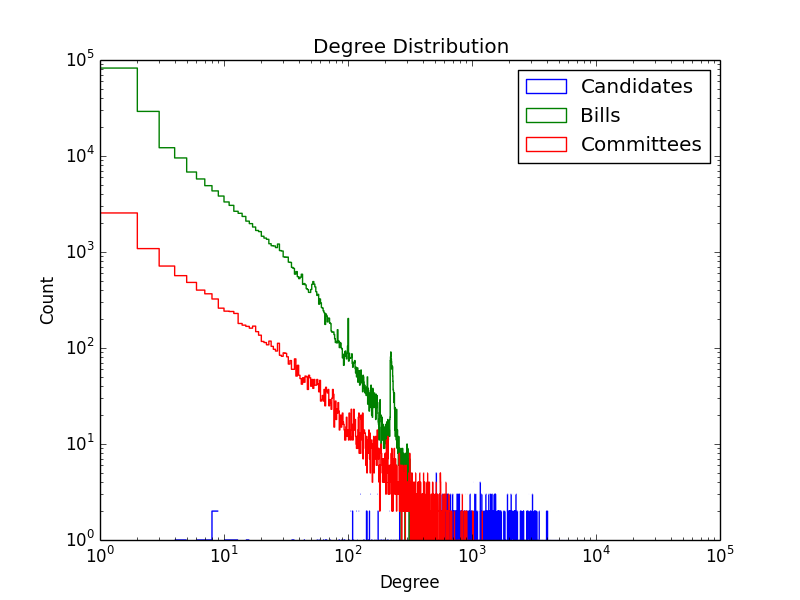
\includegraphics[width=0.5\linewidth]{overall_deg_distro}
\caption{Overall Tripartite Graph Degree Distribution on log-log scale}
\label{fig:overalldegdistro}
\end{figure}

It's perhaps more informative to look at candidates' degree distribution in the context of each subgraphs as well; so we have plotted degree distributions for both subgraphs, for legislator nodes in \ref{fig:candidate_in_bill_deg_distro} and \ref{fig:candidate_in_campaign_deg_distro}. 

\begin{figure}
\centering
\begin{minipage}{0.45\linewidth}

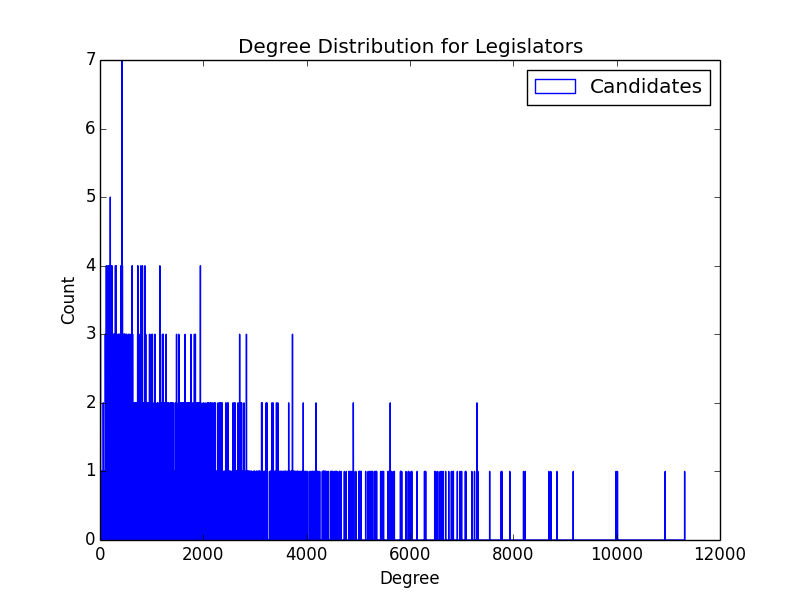
\includegraphics[width=\linewidth]{candidate_in_bill_deg_distro}
\caption{Degree Distribution of Legislator Nodes in the Bill Subgraph on a linear scale}
\label{fig:candidate_in_bill_deg_distro}
\end{minipage}\hfill
\begin{minipage}{0.45\linewidth}

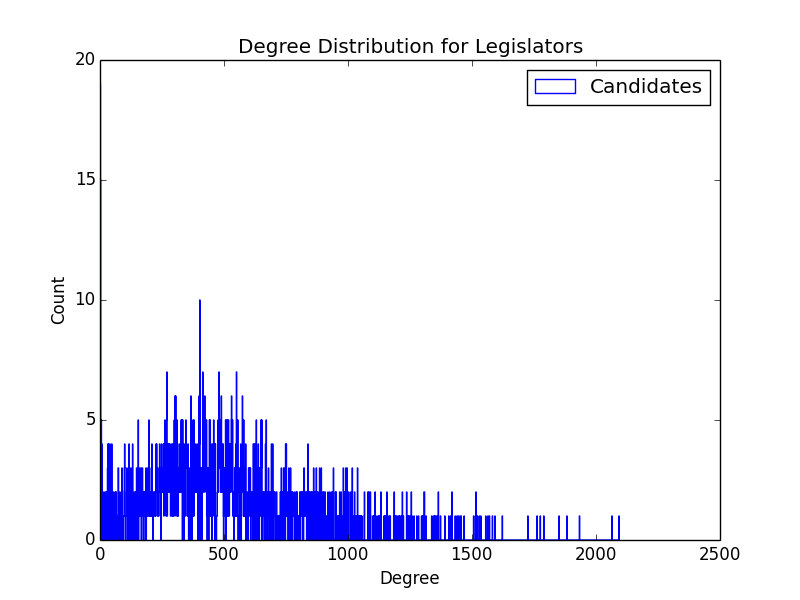
\includegraphics[width=\linewidth]{candidate_in_campaign_deg_distro}
\caption{Degree Distribution of Legislator Nodes in the Campaign Subgraph on a linear scale}
\label{fig:candidate_in_campaign_deg_distro}
 \end{minipage}
\end{figure}

Moreover, we have applied role detection to both subgraphs, with the "average legislator" as the comparison baseline and looking at the same three features as HW2: the degree of node $c$, the number of edges in the egonet of $v$, and the number of edges connects $v$'s egonet and the rest of the graph. The "average legislator" is defined as a hypothetical node with average values of the 3 features. After computing cosine similarity using $$Sim(x,y) = \frac{x\cdot{y}}{||x||_2 \cdot{||y||_2}}$$

For the bill subgraph, the role distribution is as shown in \ref{fig:billrole}; for the campaign subgraph, it's shown in \ref{fig:campaignrole}. The bill role distribution shows Legislator Node IDs {346 - Jerry Morgan of KS, 533 - Wicker Roger of MS, 1709 - Paul Simon of IL} as top 3 most similar to the "average legislator"; while the campaign subgraph shows Node IDs {322 - Thomas "Tom" McClintock of CA, 1854 - Harold Washington of IL, 369 -Beto O'Rourke of TX} as top 3 most similar to the "average legislator". None of them overlap. Clearly, the campaign subgraph's roles are not very meaningful as all nodes appear to have similar cosine similarities. We suspect that this is because we collated all the years together so that we lost data granularity in the process, and when one's been around for a while, he/she does the same thing for raising money - that is, he/she will take donations and build the money network. 

\begin{figure}
\centering
\begin{minipage}{0.45\linewidth}

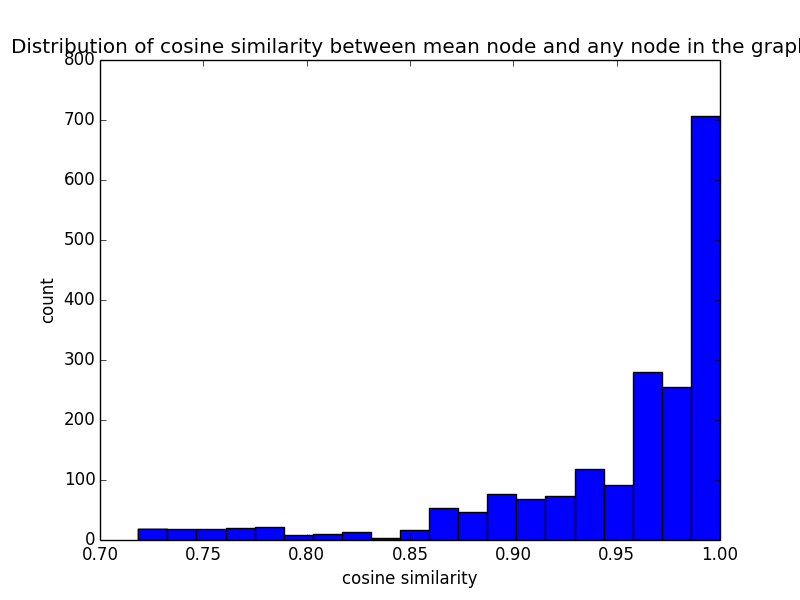
\includegraphics[width=\linewidth]{bill_role}
\caption{Roles in Bill Subgraph}
\label{fig:billrole}
\end{minipage}\hfill
\begin{minipage}{0.45\linewidth}

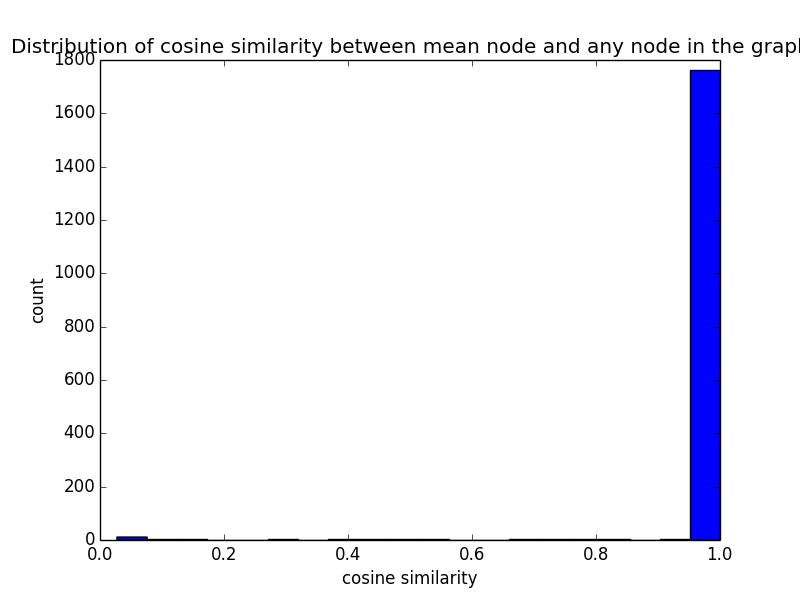
\includegraphics[width=\linewidth]{campaign_role}
\caption{Roles in Campaign Subgraph}
\label{fig:campaignrole}
 \end{minipage}
\end{figure}


Lastly, we wanted to understand how we can cut the graph efficiently, with the cut being a potential feature we can use later in link prediction in lieu of legislators' party allegiances. For the bill graph, we have the Positive Set of size  and the Negative Set, $\overline{S}$ of size 933. For the campaign subgraph, we have the Positive Set, $S$ of size 946 and the Negative Set, $\overline{S}$ of size 867, using the Clauset-Newman-Moore greedy modularity maximization provided by NetworkX. This closely resembles an even split of the aggregate two-party divide of the Congress. 

Moreover, we recognize that so far, we are treating the 36 years' data as one aggregate graph - this probably aggravates the connectedness of the graph (as over time, one tends to collaborate with most people, and to get donations from all committees on the same of the aisle). Therefore, we also isolated one batch of the tripartite graph (defined as two years' campaign contribution data plus the two following years' bill co-authorship data). It turns out that even 2 years is enough time for the graph to become densely connected. We have plotted a few degree distribution plots for Campaign Year 1999-2000 with bill data from 2001 to 2002 (the 107th Congress) in Figures \ref{fig:2000_bill_degrees_log} and \ref{fig:2000_campaign_degrees_log}. 

It holds true that the \textbf{Bill Co-authorship Graph resembles the academic collaboration graph with a power law pattern} (long tail) - the most frequent degrees are the smallest degrees, and it has a very high clustering co-efficient. It's likely due to a few reasons: politics is a tiny field that everyone knows all the issues pretty well, and can have an opinion on almost anything and therefore removing the knowledge hurdle to co-sponsor bills; Congress is a two-party system, and legislators within one party tends to co-sponsor bills together along party lines; once more than two legislators sponsor a bill, they would create a triangle thus the high clustering coefficient; yet bills come in a dime a dozen, and it's unlikely that one legislator finds it necessary or efficient to co-sponsor every single bill he/she agrees with. Moreover, sponsoring bills together can signal an alliance, making legislators consider carefully before putting down their names. 

For the \textbf{folded campaign contribution graph, it represents a typical small world pattern with high clustering coefficient}, when we look at legislators only, and a somewhat normal distribution - degrees are peaked between the smallest and the largest degrees. This makes sense as politics is a very small circle, and the national players and donors are relatively constant as they are mostly career politicians.  
\begin{figure}
\centering
\begin{minipage}{0.45\linewidth}

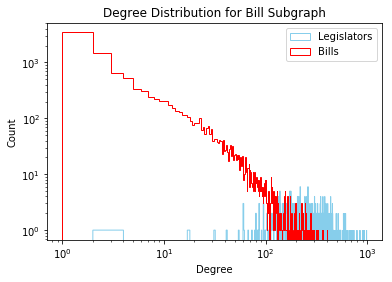
\includegraphics[width=\linewidth]{2000_bill_degrees_log}
\caption{Bill Subgraph Degree Distribution (log) for 2001-2002}
\label{fig:2000_bill_degrees_log}
\end{minipage}\hfill
\begin{minipage}{0.45\linewidth}

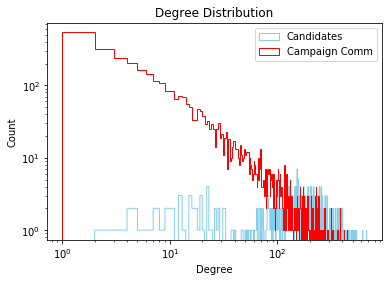
\includegraphics[width=\linewidth]{2000_campaign_degrees_log}
\caption{Campaign Subgraph Degree Distribution (log) for 1999-2000}
\label{fig:2000_campaign_degrees_log}
 \end{minipage}
\end{figure}

\subsection{Feature Selection}
Using 100th and 101st Congress, we first observed that \textbf{features from contribution amounts} always rank dead last, while contributing to slow running time of our algorithms. Thus, we removed these features first (sum and absolute difference). We then tabulated results of running F-tests for the remaining features below: 

\begin{tabular}{|l|r|}
\hline
\multicolumn{1}{|c|}{Feature} & \multicolumn{1}{c|}{F-Score} \\ \hline
Clustering Coeff Difference   & 19265.8                \\ \hline
Jaccard Index                      & 14453.4                        \\ \hline
Degree Centrality Diff                    & 10964.6                        \\ \hline
Shortest Distance            & 4615.9                    \\ \hline
Degree Difference                 & 3438.7                        \\ \hline
Clustering Coeff Sum                & 1950.9                        \\ \hline
Common Neighbors            & 1391.9                        \\ \hline
Union of Neighbors             & 1215.6                     \\ \hline
Clustering Coeff Mean              &  841.1             \\ \hline
If From Same Spectral Cluster          & 0.8                      \\ \hline
\end{tabular}

This indicates that knowing clusters generated from modularity maximization to mimic partyline is actually not helpful, which is a new learning to us. It also shows that the legislators' connectedness and the financial contribution communities they are in are important and indicative of their collaboration in office. The observation holds true when we re-ran the selection algorithm all the datasets available from the $98^{th}$ to the $112^{nd}$ Congress, with the same Top 3 Features (see Apendix A).

In order to determine how many features we should be using in logistic regression, we used grid search to determine the optimal selector percentile as shown in Figure \ref{fig:selectorpercentilegridsearch}. This shows that we should be using all the features generated so far. 
For the decision tree, we have tuned the parameter for tree-depth, in order to avoid overfitting by running a grid search as shown in Figure \ref{fig:max_depth_grid}. Therefore, we set the maximum tree depth to be 10. 

\begin{figure}
\centering
\begin{minipage}{0.5\linewidth}

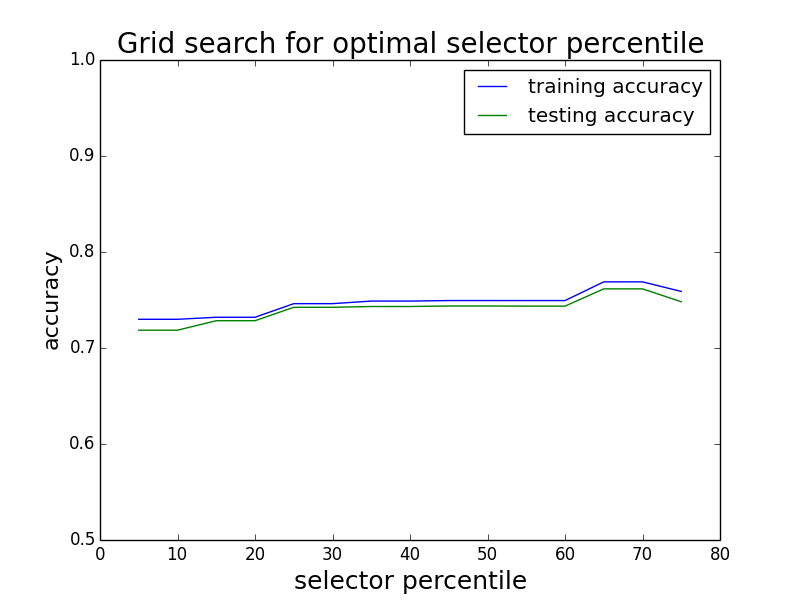
\includegraphics[width=\linewidth]{selector_percentile_grid_search}
\caption{Selector Percentile for Feature Ranking}
\label{fig:selectorpercentilegridsearch}

\end{minipage}\hfill
\begin{minipage}{0.5\linewidth}

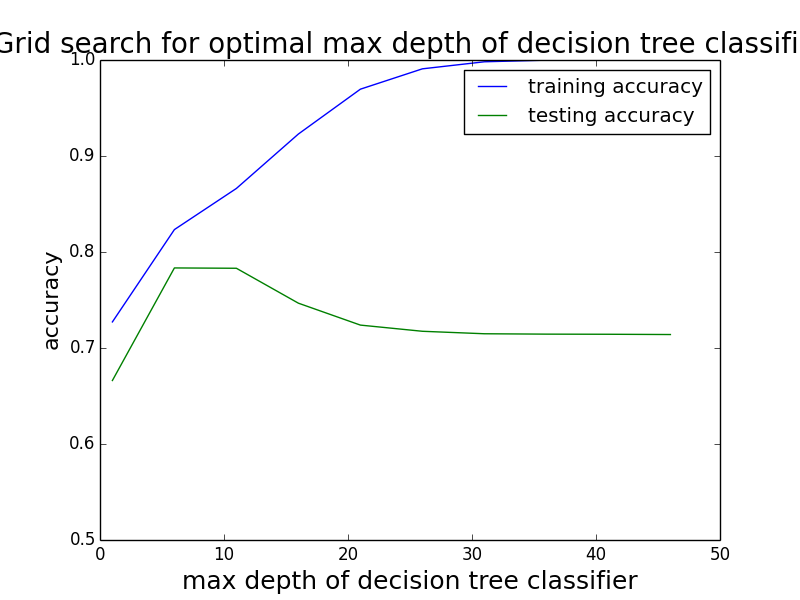
\includegraphics[width=\linewidth]{max_depth_grid}
\caption{ Grid Search for Optimal Tree Depth}
\label{fig:max_depth_grid}

 \end{minipage}
\end{figure}



\subsection{Model Performance}
We have run models in two ways: based on limited dataset (i.e. training on the $100^{th}$ Congress and test on the $101^{st}$ Congress, in what we call a one-term set), and based on richer datasets (i.e. training on the $98^{th}$ to $112^{nd}$ Congress combined graph, and test on the $113^{rd}$ to $114^{th}$ Congress combined graph). Below are our model performance in Tables \ref{tab:model1} and \ref{tab:model2}, respectively . Candidate Only Predictor uses only the Affiliated Party and Home State information from candidates, gathered form the campaign contribution data.
\begin{table}[htb]
\resizebox{\columnwidth}{!}{
\begin{tabular}{|l|r|r|}

\hline
\multicolumn{1}{|c|}{Model} & \multicolumn{1}{c|}{Train Accuracy} & \multicolumn{1}{c|}{Test Accuracy} \\ \hline
Naive Baseline  & 0.695      & 0.695         \\ \hline
Candidate Party/State  & 0.695      & 0.698         \\ \hline
Logistic Regression & 0.786      & 0.774         \\ \hline
Decision Tree & 0.854      & 0.794         \\ \hline
Logistic Reg w/ Node2Vec & 0.728      & 0.728         \\ \hline
\end{tabular}
}
\caption{Model Performance for Limited Dataset}
  \label{tab:model1}
\end{table}

\begin{table}[htb]
\resizebox{\columnwidth}{!}{
\begin{tabular}{|l|r|r|}

\hline
\multicolumn{1}{|c|}{Model} & \multicolumn{1}{c|}{Train Accuracy} & \multicolumn{1}{c|}{Test Accuracy} \\ \hline
Naive Baseline  & 0.697      & 0.691         \\ \hline
Candidate Party/State  & 0.695      & 0.698         \\ \hline
Logistic Regression & 0.748      & 0.714         \\ \hline
Decision Tree & 0.795      & 0.740         \\ \hline
\end{tabular}
}
\caption{Model Performance for All Datasets Combined}
  \label{tab:model2}
\end{table}

To visualize models' accuracy in terms of true positives and true negatives, we have plotted confusion matrices for the limited dataset in Figures \ref{fig:confusion_tree_limited} and \ref{fig:logreg_limited}. %(confusion matrices for all datasets can be found in Appedix B)

\begin{figure}
\centering
\begin{minipage}{0.48\linewidth}

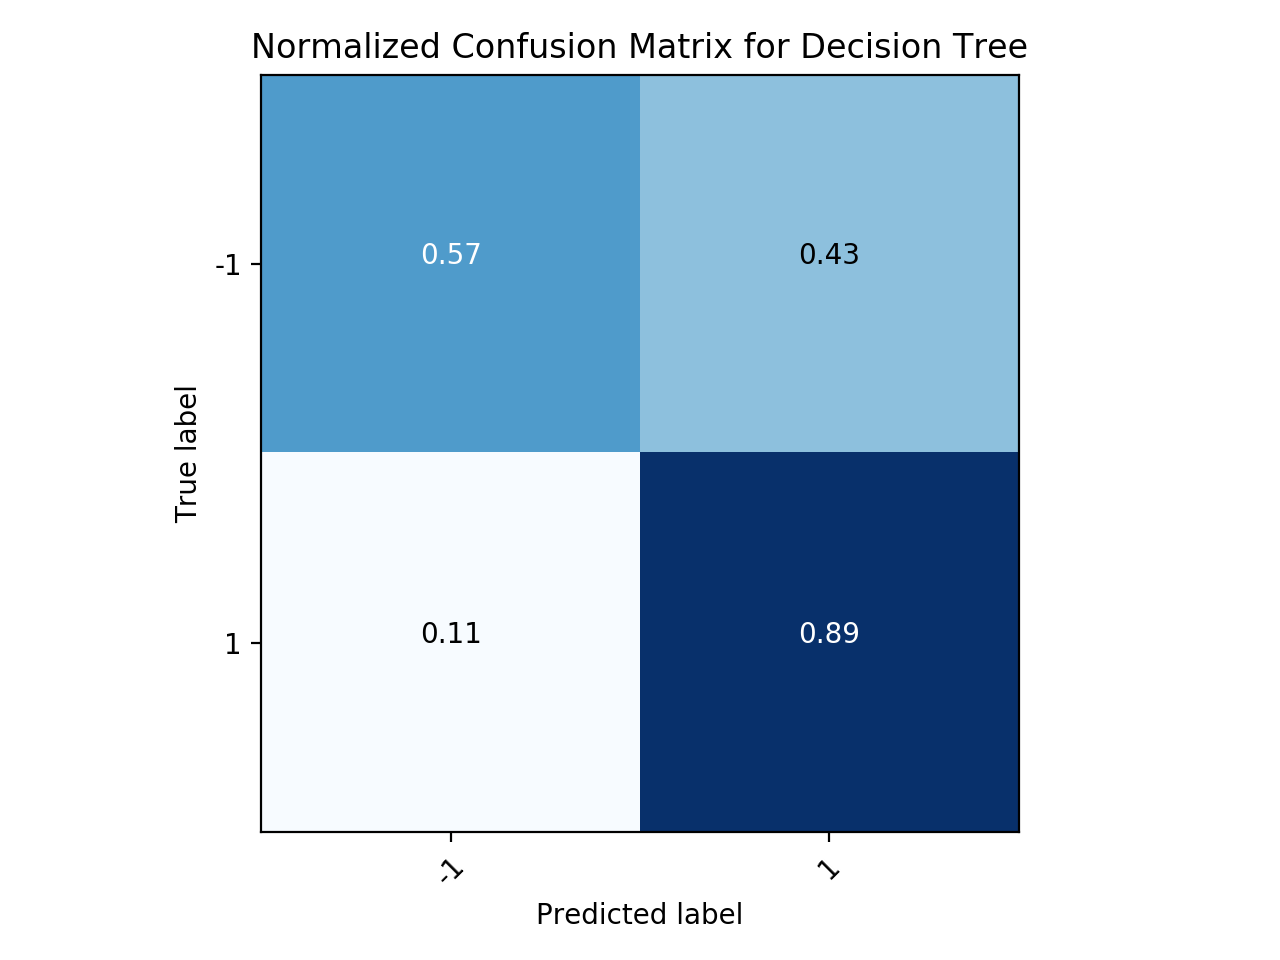
\includegraphics[width=\linewidth]{confusion_tree_limited}
\caption{Confusion Matrix for Decision Tree in Limited Dataset}
\label{fig:confusion_tree_limited}
\end{minipage}\hfill
\begin{minipage}{0.48\linewidth}

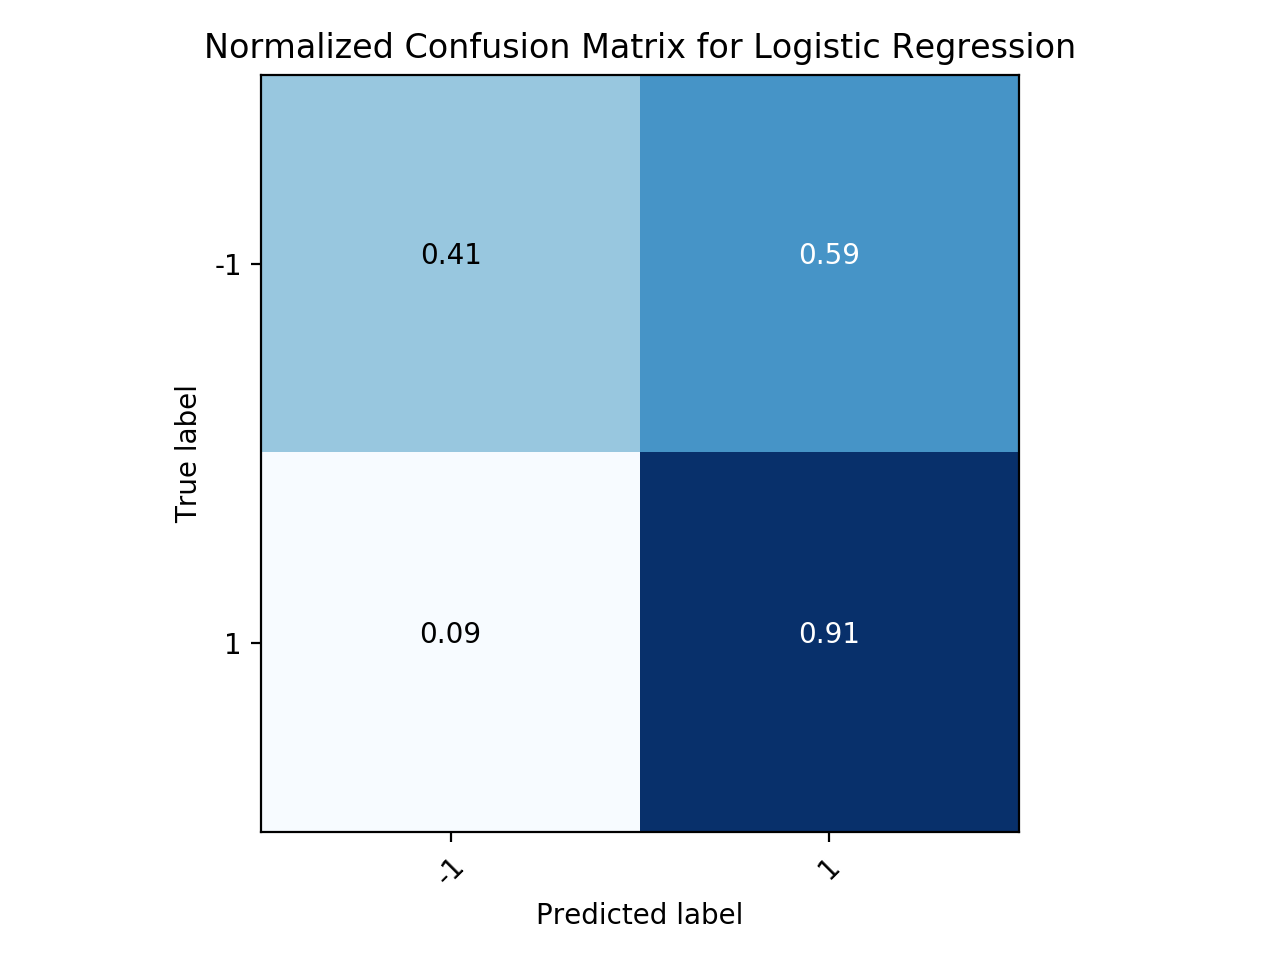
\includegraphics[width=\linewidth]{logreg_limited}
\caption{Confusion Matrix for Logistic Regression in Limited Dataset}
\label{fig:logreg_limited}
 \end{minipage}
\end{figure}

\subsection{Discussion}
It's interesting to note that knowing candidates' party and home state information does not lead to a better model when compared to the naive baseline, and using node2vec as we tried in this paper does not help either. Decision tree performed neck and shoulders above the rest, and a better performance in avoiding false positives and false negatives too when compared to logistic regression. This lends support to our hypothesis that money has a big influence in political collaboration: knowing the network structures of candidates' campaign donation graphs, we can reliably predict whom they wil collaborate with when elected, in the form of co-sponsoring bills. 
\section{Conclusion}
US Congressional Politics is indeed a small world: legislators are connected to other legislators via common donors and co-authorship on bills. We have identified the academic collaboration network-like pattern for bill co-authorship data, and a "small world" pattern among legislators, with consistently high clustering coefficients. Moreover, it does appear that "money moves politics": using features learned from campaign donation networks, we can confidently predict if two legislators will later collaborate on bills together - easily beating a naive baseline. In paricular, decision tree model performed very well to give us $82\%$ accuracy. 

This sheds new light on understanding politicians' behavior in Congress. Among many potential application, we now have a reliable way to predict if an elected candidate's campaign trail promises will likely carry through, by looking at whose money he/she has taken from, and with what other politicians does one share donors with. 

\section{Acknowledgement}
\textbf{Yi}: Cleaning and processing the bill co-authorship data, coming up and coding the algorithms, problem formulation, running tests, tabulating final results, editing the report. \\
\textbf{Eddie}: Plotting graphs during data analysis, cleaning and processing the campaign contribution data, conducting network descriptive analysis, problem formulation, writing up the report. \\
We'd like to thank the CS224W TA stuff for helpful feedback to our project prosal and milestone report. 

% trigger a \newpage just before the given reference
% number - used to balance the columns on the last page
% adjust value as needed - may need to be readjusted if
% the document is modified later
%\IEEEtriggeratref{8}
% The "triggered" command can be changed if desired:
%\IEEEtriggercmd{\enlargethispage{-5in}}

% references section
\bibliography{ref}
\bibliographystyle{plain}

\appendix
\section{Feature Ranking with All Datasets}
\begin{tabular}{|l|r|}
\hline
\multicolumn{1}{|c|}{\textbf{Feature}} & \multicolumn{1}{c|}{\textbf{F-Score}} \\ \hline
Jaccard Index                      & 180126.1                       \\ \hline
Degree Centrality Diff                    & 99775.0                    \\ \hline
Clustering Coeff Difference   & 65108.8              \\ \hline
Shortest Distance            & 49727.1                   \\ \hline
Common Neighbors            & 22229.7                     \\ \hline
Clustering Coeff Sum                & 19472.1                       \\ \hline
Union of Neighbors             & 9183.6                     \\ \hline
Degree Difference                 & 8650.4                        \\ \hline
Clustering Coeff Mean              &  7026.5             \\ \hline
Congress Term          & 3.6                    \\ \hline
If From Same Spectral Cluster          &2.6                      \\ \hline
\end{tabular}

%\section{Confusion Matrices for All Datasets}


\end{document}


